\documentclass[
  11pt,
  letterpaper,
   addpoints,
   answers
  ]{exam}

\usepackage{../exercise-preamble}

\begin{document}

\noindent
\begin{minipage}{0.47\textwidth}

\includegraphics[width=\textwidth]{../fcfm_die}
\end{minipage}
\begin{minipage}{0.53\textwidth}
\begin{center} 
\large\textbf{Fundamentos de control de sistemas} (EL4111-1) \\
\large\textbf{Pauta auxiliar 12} \\
\small Prof.~Roberto Cardenas Dobson\\
\small Prof.~Aux.~Osvaldo Jimenez - Erik Sáez\\
\small Ayudantes.~Simon Arenas- Juan Pablo Baez - Francisco Garces - Sofia Ibarra\\
\end{center}
\end{minipage}

\vspace{0.5cm}
\noindent
\vspace{.85cm}
\section{Resumen}
Un sistema de control se puede representar mediante un modelo de espacio de estados, el cual se puede expresar como:
\begin{align}
    \dot{x}(t) &= Ax(t) + Bu(t) + \text{Perturbaciones} \\
    y &= Cx(t) + Du(t) + \text{Perturbaciones}
\end{align}
Consideramos el caso continuo, como recordatorio tenemos que:
\begin{itemize}
    \item \textbf{x(t):} Representa el vector de estados del sistema el cual se entiende como las variables internas del sistema que describen su comportamiento.
    \item \textbf{u(t):} Representa el vector de entradas del sistema, es decir, las señales de control que se aplican al sistema (\textit{La variable que podemos manipular}).
    \item \textbf{y(t):} Representa el vector de salidas del sistema, es decir, las señales que se obtienen como respuesta del sistema.
    \item \textbf{A, B, C, D:} Representan las matrices de estado del sistema, las cuales se obtienen a partir de las ecuaciones diferenciales que describen el sistema en particular.
\end{itemize}
Esta representacion esta planteada para un sistema \textbf{lineal} en caso de no ser asi, se debe linealizar el sistema utilizando Taylor para poder aplicar este modelo. (\textit{Es importante entender que la linealizacion se realiza en torno a un punto de operacion y que en un sistema pueden existir multiples, sea por ejemplo el caso de un pendulo unido a una barra firme donde tenemos dos posiciones de estabilidad siendo una estable y otra inestable}).
\subsection{Control por re-ubicacion de polos}
Recordemos que los polos de un sistema en variables fisicas son los valores propios de la matriz A, por lo que si se desea re-ubicar los polos del sistema se debe realizar un diseño de control por realimentacion de estados, el cual se basa en el calculo de la matriz de realimentacion K, la cual se obtiene a partir de la ecuacion caracteristica del sistema. (\textit{Ademas se debe recordar que los si todos los valores propios de la matriz A son negativos, el sistema se dice que es estable}). Retomemos el sistema lineal considerando que D=0
\begin{align}
    \dot{x(t)} &= Ax(t) + Bu(t) \\
    y &= Cx(t)
\end{align}
Luego si se implementa una entrada tal que $u(t) = R(s) -Kx(s)$ tendremos que reemplazando en la ecuacion de estado se obtiene:
\begin{align}
    \dot{x}(t) &= Ax(t) + B(R(s) - Kx(s))\\
    \dot{x}(t) &= (A - BK)x(t) + BR(s)
\end{align}
Por lo tanto tenemos que la nueva matriz de estado sera $A_{c} = A - BK$, por lo que si se desea re-ubicar los polos del sistema se debe calcular la matriz K tal que los valores propios de la matriz $A_{c}$ sean los deseados. Previamente se debe verificar que el sistema sea controlable para poder aplicar esta idea, esto se logra con la matriz de controlabilidad $\zeta$ la cual se obtiene como:
\begin{align}
    \zeta =
    \begin{bmatrix}
         B & AB & A^{2}B + \dots & + A^{n-1}B
    \end{bmatrix}
\end{align}
Para determinar si el sistema es controlable se debe verificar que el sistema sea de rango completo, una forma de obtener esto es verificando si el determinante de la matriz de controlabilidad es distinto de 0. (\textit{Otra forma rapida y equivalente si la matriz es de rango completo es ver si filas y columnas son LI, mas forma las adjunto en el apunte de dinamicos \href{https://www.u-cursos.cl/ingenieria/2024/1/EL3204/1/material_docente/detalle?id=7719473}{link}}).Algunos detalles de lo anterior son los siguientes:
\begin{itemize}
    \item Si el estado es no controlable pero es estable podriamos estar en problemas si la dinamica es muy lenta
    \item Si el estado no es controlable y su funcion de transferencia es inestable, entonces definitivamente estamos en problemas
    \item Hasta el momento no hemos considerado el cero error a estado estacionario, esto se logra con estados integrales.
    \item Una forma de obtener K es a través de la forma canonica controlable
\end{itemize}
\newpage
\begin{questions}
%----------------------------------------------
    \question 
    El filtro más utilizado para conectar sistemas de generación distribuida es el L-C-L, debido a que esta topología tiene mejor razón potencia/volumen. Sin embargo, debido a un problema de costos, una empresa decide comercializar una inusual solución de bajo costo y menor eficiencia consistente en el sistema L-C-R que se muestra en la figura. En el esquema mostrado \( V_c \) es la tensión manipulada y \( V_{\text{red}} \) es la tensión de la red (que no puede ser manipulada). Los valores de los parámetros son \( L = 1\,\text{mH} \), \( C = 30\,\mu\text{F} \), \( R = 1\,\Omega \). La bobina \( L \) tiene una resistencia intrínseca de \( 0.3\,\Omega \). La salida del sistema es la corriente \( i_2 \).

    \begin{figure}[h!]
        \centering
        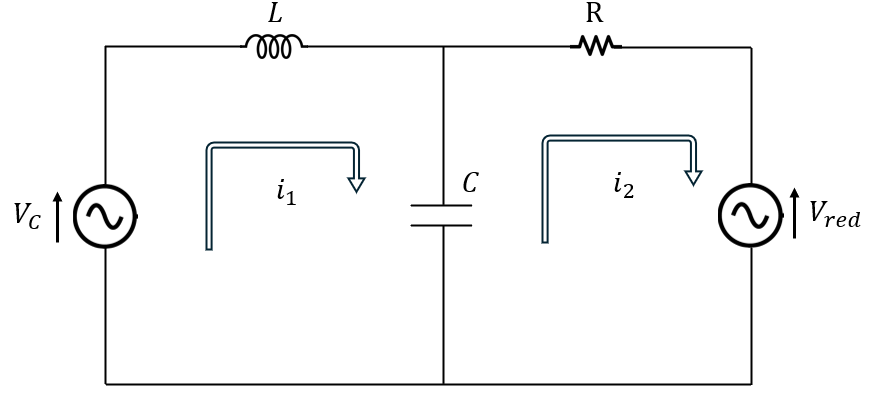
\includegraphics[width=0.5\textwidth]{Auxiliar_12_1}
        \caption{Sistema de generación conectado mediante filtro LCL a la red.}
    \end{figure}

    \begin{enumerate}
        \item[(a)] Escriba las ecuaciones de estado del sistema de la Figura 1 identificando todas las matrices. Encuentre los valores propios actuales del sistema.
        
        \item[(b)] Escriba las ecuaciones de estado correspondientes al sistema que se muestra en la Fig.1 (identificando todas las matrices y las referencias), considerando control integral en la corriente \( i_1 \). Si el sistema es controlable, diseña utilizando la forma canónica de control la realimentación de estado necesaria para obtener los siguientes valores propios: \(-100, -100 \pm j100\). El sistema de control debe implementarse utilizando variables de estado físicas.
    \end{enumerate}
%----------------------------------------------
\begin{solution}
    \subsection*{Resolucion 1.1}
    Se busca obtener las ecuaciones en variables de estado del sistema de figura 1, es decir:
    \begin{align}
        \dot{x}(t) &= Ax(t) + Bu(t) + \text{Perturbaciones} \\
        y &= Cx(t) + Du(t) + \text{Perturbaciones}
    \end{align}
    Retomando el sistema visto en la figura 1. tenemos que este circuito puede ser resuelto mediante metodo de mallas, obteniendo el siguiente esquema:
    \begin{center}
        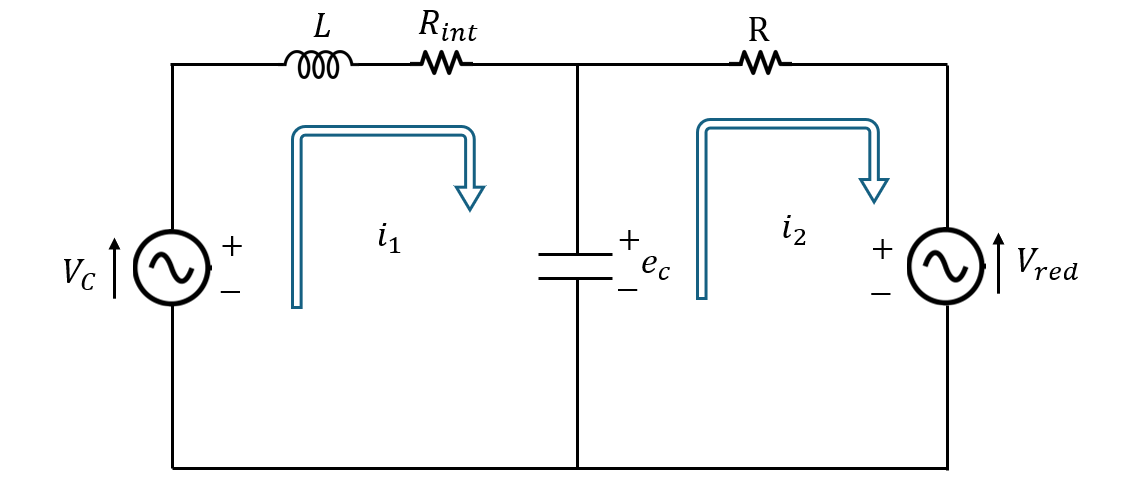
\includegraphics[width=0.6\textwidth]{Auxiliar_12_2}
    \end{center}
    \begin{center}
        \textbf{Figura 1:} Circuito electrico
    \end{center}
    La resistencia intrinseca ($r_{int}$) esta asocada a la bobina, luego tenemos que las ecuaciones de las malla 1 y 2 vendran dadas lo siguiente:
    \begin{align}
        -V_{c} + V_{L} + R_{int} \cdot i_{1} + e_{c}&= 0 \\
        -e_{c}  + R\cdot i_{2} + V_{red} &= 0
    \end{align}
    Luego tenemos que $V_{l} = L \frac{di_{1}}{dt}$ y $i_{c}= C\frac{de_{c}}{dt}$.Ademas dada la polaridad del condensador es posible imponer que:
    \begin{align}
        i_{c} = i_{1} - i_{2}\\
        i_{2} = i_{1} + i_{c}
    \end{align}
    Luego tenemos que:
    \begin{align}
        -V_{c} + V_{L} + R_{int} \cdot i_{1} + e_{c}&= 0\\
        V_{L} &= V_{c} - R_{int} \cdot i_{1} - e_{c}\\
        L \frac{di_{1}}{dt} &= V_{c} - R_{int} \cdot i_{1} - e_{c}\\
        \frac{di_{1}}{dt} &= \frac{V_{c}}{L} - \frac{R_{int}}{L} \cdot i_{1} - \frac{e_{c}}{L} 
    \end{align}
    Esto nos permite obtener la primera ecuacion de estado, mientras que por otro lado:
    \begin{align}
        -e_{c} + R\cdot i_{2} + V_{red} &= 0\\
        i_{2} &= \frac{e_{c} - V_{red}}{R}\\ 
    \end{align}
    Se reemplaza en:
    \begin{align}
        i_{1} &= i_{2} + i_{c}\\
        i_{1} &= \frac{e_{c} - V_{red}}{R} + i_{c}\\
        i_{1} &= \frac{e_{c} - V_{red}}{R} + C\frac{de_{c}}{dt}\\
        \frac{de_{c}}{dt} &= \frac{i_{1}}{C} - \frac{e_{c}}{RC}  + \frac{V_{red}}{RC}
    \end{align}
    De esta manera se obtiene la segunda ecuacion de estado. Luego se tiene que la formulacion en variables de estado correspondera a:
    \begin{align}
        \begin{bmatrix}
            \dot{i_{1}}\\
            \dot{e_{c}}
        \end{bmatrix}
        &=
        \begin{bmatrix}
            -\frac{R_{int}}{L} & \frac{-1}{L}\\
            \frac{1}{C} & -\frac{1}{RC}
        \end{bmatrix}
        \begin{bmatrix}
            i_{1}\\
            e_{c}
        \end{bmatrix}
        +
        \begin{bmatrix}
            \frac{1}{L}\\
            0
        \end{bmatrix}
        V_{c}
        +
        \begin{bmatrix}
            0\\
            \frac{1}{RC}
        \end{bmatrix}
        V_{red}
    \end{align}
    De esta manera es posible identificar cada matriz como:
    \begin{align}
        A &=
        \begin{bmatrix}
            -\frac{R_{int}}{L} & \frac{-1}{L}\\
            \frac{1}{C} & -\frac{1}{RC}
        \end{bmatrix}\\
        B &=
        \begin{bmatrix}
            \frac{1}{L}\\
            0
        \end{bmatrix}
    \end{align}
        Ademas notamos que las perturbaciones van asociada a $V_{red}$, recordemos que $v_{c}$ no es una perturbacion dado que corresponde a la variable de entrada o manipulable:
        \begin{align}
            \begin{bmatrix}
                0\\
                \frac{1}{RC}
            \end{bmatrix}
            V_{red}
        \end{align}
        Con lo que ya es posible formular el sistema como:
        \begin{align}
            \dot{x}(t0) &= Ax(t) + Bu(t) + \text{Perturbaciones} 
        \end{align}
        Por otro lado se tiene que la salida del sistema es la corriente \( i_2 \) (\textit{Por enunciado}), por lo que se tiene que:
        \begin{align}
            y &= Cx(t) + Du(t) + \text{Perturbaciones}
        \end{align}
        Volviendo sobre lo anterior se define la salida como \( y = i_{2} \), por lo que se tiene que:
        \begin{align}
            i_{2} &= \frac{e_{c} - V_{red}}{R}\\
            i_{2} &= \frac{1}{R} \cdot e_{c} - \frac{V_{red}}{R}
        \end{align}
        Luego en formato de matriz tendremos que:
        \begin{align}
            y &=
            \begin{bmatrix}
                0 & \frac{1}{R}
            \end{bmatrix}
            \begin{bmatrix}
                i_{1}\\
                e_{c}
            \end{bmatrix}
            -\frac{V_{red}}{R}
        \end{align}
        De esta manera se logra identificar C yD como las matrices:
        \begin{align}
            C &=
            \begin{bmatrix}
                0 & \frac{1}{RC}
            \end{bmatrix}\\
            D &= 0
        \end{align}
        Considerando los valores del enunciado dados por \( L = 1\,\text{mH} \), \( C = 30\,\mu\text{F} \), \( R = 1\,\Omega \) y \( R_{int} = 0.3\,\Omega \) se tiene que reemplazando los valores de las matrices, se tendra:
        \begin{align}
            A &=
            \begin{bmatrix}
                -300 & -1000\\
                \frac{100000}{3} & -\frac{100000}{3}
            \end{bmatrix}\\
            B &=
            \begin{bmatrix}
                1000\\
                0
            \end{bmatrix}\\
            C &=
            \begin{bmatrix}
                0 & \frac{100000}{3}
            \end{bmatrix}\\
        \end{align}
        Por otro lado tendremos que la salida $i_{2}$ correspondera a:
        \begin{align}
            y &=
            \begin{bmatrix}
                0 & 1
            \end{bmatrix}
            \begin{bmatrix}
                i_{1}\\
                e_{c}
            \end{bmatrix}
            -\frac{V_{red}}{1}
        \end{align}
        Debido a que se busca determinar los polos del sistema, sera equivalente a determinar los valores propios de la matriz A, por lo que se tiene que:
        \begin{align}
            \text{det}(A - \lambda I) &= 0\\
            \text{det}
            \begin{bmatrix}
                -300 - \lambda & -1000\\
                \frac{100000}{3} & -\frac{100000}{3} - \lambda
            \end{bmatrix}
            &= 0\\
            (-300 - \lambda)(-\frac{100000}{3} - \lambda) - (-1000)(\frac{100000}{3}) &= 0\\
            \lambda^{2} + \frac{100900}{3}\lambda - \frac{130000000}{3} &= 0
        \end{align}
        De esta manera al resolver la ecuacion cuadratica se obtiene que los valores propios del sistema son:
        \begin{align}
            \lambda_{1} =  - 1342,39\\
            \lambda_{2} =  -32291,39
        \end{align}
        Se observa ademas que el sistema es estable dado que los valores propios son negativos.
        \subsection*{Resolucion 1.2}
        Por enunciado se menciona que se busca obtener un control integral de la corriente $i_{1}$, estos controles cumplen con algunas caracteristicas dadas por:
        \begin{itemize}
            \item Se debe agregar uno por cada variable de estado que se quiera obtener CEEE o control integral a una entrada escalon
            \item No siempre es posible obtener un control integral para todas las variables de estado
            \item Estos estados no son observables
        \end{itemize}
        Luego tenemos que el sistema en variables de estado con control integral sera:
        \begin{align}
            \begin{bmatrix}
                \dot{i_{1}}\\
                \dot{e_{c}}\\
                \dot{X_{i}}
            \end{bmatrix}
            &=
            \begin{bmatrix}
                -\frac{R_{int}}{L} & \frac{-1}{L} & 0\\
                \frac{1}{C} & -\frac{1}{RC} & 0\\
                1 & 0 & 0
            \end{bmatrix}
            \begin{bmatrix}
                i_{1}\\
                e_{c}\\
                X_{i}
            \end{bmatrix}
            +
            \begin{bmatrix}
                \frac{1}{L}\\
                0\\
                0
            \end{bmatrix}
            V_{c}
            +
            \begin{bmatrix}
                0\\
                \frac{1}{RC}\\
                0
            \end{bmatrix}
            V_{red}
            +
            \begin{bmatrix}
                0\\
                0\\
                -1
            \end{bmatrix}
            i^{*}_{1}
        \end{align}
        Se obtienen las nuevas matrices A', B' y C', Es importante notar algunos aspectos de la mismas. Para la nueva matriz A al adicionar un nuevo estado, se genera por tanto una nueva fila y columna en la matriz A, donde en la fila se adiciona un 1 en la variable donde se busque obtener el control integral (\textit{Que en este caso se hace unicamente para la corriente dado que por ejemplo no queremos control integral para $e_{c}$}) y ademas se agrega una ultima columna que sirve para setear el valor de referencia de la variable de estado que se busca controlar.

        Luego se debe verificar si el sistema es controlable, para ello se debe verificar si la matriz de controlabilidad es de rango completo, recordemos que esta viene de manera general por:
        \begin{align}
            \zeta =
            \begin{bmatrix}
                 B & AB & A^{2}B + \dots & + A^{n-1}B
            \end{bmatrix}
        \end{align}
        De esta manera tenemos que que reemplazando valores:
        \begin{align}
            B' = 
            \begin{bmatrix}
                10^{3}\\
                0\\
                0
            \end{bmatrix}
            A'B' = 
            \begin{bmatrix}
                -3 \cdot 10^{5}\\
                \frac{10^{8}}{3}\\
                1000
            \end{bmatrix}
            A'^{2}B' = 
            \begin{bmatrix}
                -3.324 \cdot 10^{10}\\
                -1.121 \cdot 10^{12}\\
                -3\cdot 10^{5}
            \end{bmatrix}
        \end{align}
        Luego se tiene que la matriz de controlabilidad sera:
        \begin{align}
            \zeta =
            \begin{bmatrix}
                10^{3} & -3 \cdot 10^{5} & -3.324 \cdot 10^{10}\\
                0 & \frac{10^{8}}{3} & -1.121 \cdot 10^{12}\\
                0 & 1000 & -3\cdot 10^{5}
            \end{bmatrix}
        \end{align}
        Para verificar si la matriz es de rango completo se debe verificar si el determinante de la matriz es distinto de 0, en caso de serlo se tiene que el sistema es controlable. Luego se tiene que:
        \begin{align}
            det(\zeta) = 1.11 \cdot 10^{18} \neq 0
        \end{align}
        Por lo que podemos concluir que el sistema es controlable. Existen variadas formas equivalente de verificar si el sistema es controlable (\textit{Otra forma rapida y equivalente si la matriz es de rango completo es ver si filas y columnas son LI, mas forma las adjunto en el apunte de dinamicos \href{https://www.u-cursos.cl/ingenieria/2024/1/EL3204/1/material_docente/detalle?id=7719473}{link}
        }). Se busca expresar el sistema en su forma canonica controlable, es decir:
        \begin{align}
            A_{c}=
            \begin{bmatrix}
                -a_{1} & -a_{2} & -a_{3} & \dots & -a_{n}\\
                1 & 0 & 0 & \dots & 0\\
                0 & 1 & 0 & \dots & 0\\
                \vdots & \vdots & \vdots & \ddots & \vdots\\
            \end{bmatrix}
            B_{c}
            \begin{bmatrix}
                1\\
                0\\
                \vdots\\
                0
            \end{bmatrix}
        \end{align}
        Dado que ahora consideramos el sistema con la matriz con control integral, se tendra que su ecuacion caracteristica sera dada por:
        \begin{align}
            \text{det}(A_{CI} - \lambda I) = 0
        \end{align}
        Luego se tiene que:
        \begin{align}
        -\lambda^{3} - 33633.33\lambda^{2} - 4.33 \cdot 10^{7} \lambda &= 0\\
        P(\lambda) = \lambda^3 + \underbrace{33633.33}_{a_1}\lambda^2 + \underbrace{4.33 \cdot 10^7}_{a_2}\lambda + \underbrace{0}_{a_3} = 0
        \end{align}
        Con lo que la forma canonica controlable sera:
        \begin{align}
            \dot{X}_c =
            \begin{bmatrix}
            \overbrace{-33633.33}^{-a_1} & \overbrace{-4.33 \cdot 10^7}^{-a_2} & \overbrace{0}^{-a_3} \\
            1 & 0 & 0 \\
            0 & 1 & 0
            \end{bmatrix}
            \cdot X_c +
            \begin{bmatrix}
            1 \\
            0 \\
            0
            \end{bmatrix}
            \cdot u_c
        \end{align}
        Es importante tener el cuidado con los signos. Dado que se busca que el sistema tenga polos en \( s = -100, -100 \pm j100 \) se busca llegar a lo siguiente:
        \begin{align}
            P^{*}(\lambda) = \lambda^3 + 
            \overbrace{300}^{\alpha_1} \lambda^2 + 
            \overbrace{40000}^{\alpha_2} \lambda + 
            \overbrace{2000000}^{\alpha_3} = 0
        \end{align}
        Mientras que lo que se tiene actualmente es:
        \begin{align}
            P(\lambda) = \lambda^3 + 
            \overbrace{33633.33}^{a_1} \lambda^2 + 
            \overbrace{4.33 \cdot 10^7}^{a_2} \lambda + 0
        \end{align}
        Luego dado que queremos obtener $\alpha$ y estamos ubicados en a , tendremos que:
        \begin{align}
            -\alpha_{1} = -a_{1} + -k_{1}\\
            -\alpha_{2} = -a_{2} + -k_{2}\\
            -\alpha_{3} = -a_{3} + -k_{3}
        \end{align}
        Con lo que reemplazando se logra obtener:
        \begin{align}
            k_{1} = 33333.33\\
            k_{2} = -4.326 \cdot 10^{7}\\
            k_{3} = 2 \cdot 10^{6}
        \end{align}
        Con lo que la matriz de realimentacion sera:
        \begin{align}
            K^{c} = 
            \begin{bmatrix}
                k_{1} & k_{2} & k_{3}
            \end{bmatrix}
        \end{align}
        Reemplazando los valores obtenidos anteriormente:
        \begin{align}
            K^{c} = 
            \begin{bmatrix}
                33333.33 & -4.326 \cdot 10^{7} & 2 \cdot 10^{6}
            \end{bmatrix}
        \end{align}
        Si bien se obtiene la matriz de realimentacion K, es importante recordar que el sistema se encuentra en el espacio canonico controlable, por lo que se debe volver a las variables fisicas utilizando la matriz de transformacion, la cual viene dada por::
        \begin{align}
            K = K^{c} \cdot T
        \end{align}
        Donde T se logra obtener como:
        \begin{align}
            T = \zeta^{c} \cdot \zeta^{-1}
        \end{align}
        Donde la primera corresponde a la matriz controlable pero del espacio canonico, eso quiere decir que:
        \begin{align}
            \zeta^{c} =
            \begin{bmatrix}
                B_{c} & A_{c}B_{c} & A_{c}^{2}B_{c}
            \end{bmatrix}
        \end{align}
        Donde los valores vendran dados por:
        \begin{align}
            B_{c} = 
            \begin{bmatrix}
                1\\
                0\\
                0
            \end{bmatrix}\\
            A_{c}B_{c} = 
            \begin{bmatrix}
                -33633.33\\
                1\\
                0
            \end{bmatrix}\\
            A_{c}^{2}B_{c} = 
            \begin{bmatrix}
                1.088 \cdot 10^{9}\\
                -33633.33\\
                1
            \end{bmatrix}
        \end{align}
        Mientra que $\zeta$ es el obtenido con anterioridad, por lo tanto tendremos que:
        \begin{align}
            T = \zeta^{c} \cdot \zeta^{-1} =
            \begin{bmatrix}
                0.001 & -0.001 & 0.0072\\
                0 & 3 \cdot 10^{-8} & -9.991 \cdot 10^{-8}\\
                0 & -9 \cdot 10^{-13} & 3 \cdot 10^{-8}
            \end{bmatrix} 
        \end{align}
        Finalmente es posible obtener la retro-alimentacion en variables fisicas como:
        \begin{align}
            K= K^{c} \cdot T =
            \begin{bmatrix}
                33333.33 & -4.326 \cdot 10^{7} & 2 \cdot 10^{6}
            \end{bmatrix}
            \cdot
            \begin{bmatrix}
                0.001 & -0.001 & 0.0072\\
                0 & 3 \cdot 10^{-8} & -9.991 \cdot 10^{-8}\\
                0 & -9 \cdot 10^{-13} & 3 \cdot 10^{-8}
            \end{bmatrix}
        \end{align}
        Dando como resultado lo siguiente:
        \begin{align}
            K = 
            \begin{bmatrix}
                -33.33 & 32.04 & -235.6
            \end{bmatrix}
        \end{align}
        Con lo que finalmente se obtiene la matriz de retroalimentacion K que permite controlar el sistema a los polos deseados.
\end{solution}
%----------------------------------------------
    \question 
    Se tienen las siguientes funciones de transferencia:
    \begin{center}
    \begin{tikzpicture}[auto, node distance=2cm, >=latex']

        % Nodes
        \node [coordinate] (input) {};
        \node [draw, rectangle, minimum width=2.5cm, minimum height=1.5cm, right of=input, node distance=2cm] (block1) {\(\frac{5}{s+3}\)};
        \node [draw, rectangle, minimum width=2.5cm, minimum height=1.5cm, right of=block1, node distance=3.5cm] (block2) {\(\frac{5}{s+6}\)};
        \node [coordinate, right of=block2, node distance=2cm] (output) {};
    
        % Connections
        \draw[->] (input) -- (block1);
        \draw[->] (block1) -- (block2);
        \draw[->] (block2) -- (output);
    
        % Labels (manually adjustable positions)
        \node at ($(input) + (-0.5, 0.5)$) {\(V(s)\)}; % Adjust (-0.5, 0.5) to move V(s)
        \node at ($(block1.east) + (0.5, 0.5)$) {\(I(s)\)}; % Adjust (1.5, 0.5) to move I(s)
        \node at ($(block2.east) + (1, 0.5)$) {\(T(s)\)}; % Adjust (2.0, 0.5) to move T(s)
    
    \end{tikzpicture}
    \end{center}
    Donde \( i(s) \) representa la corriente y \( T(s) \) el torque medio. Se desea analizar el sistema utilizando técnicas de control en variables de estado. Para ello se pide:
    
    \begin{enumerate}
        \item[(a)] Encuentre la representación física del sistema (con \( i(t) \) y \( T(t) \)). Asuma que control integral es requerido en \( T(t) \). Identifique las matrices \( A, B, C, D \) en el sistema considerando el control integral añadido.
        
        \item[(b) \textbf{(Propuesto)}] Verifique si el sistema es controlable y diseñe por realimentación de estados un controlador que entregue polos en \( s = -10 \) y \( s = -5 \pm j5 \). Utilice la forma canónica de control en su diseño.
    \end{enumerate}
%----------------------------------------------
\begin{solution}
\subsection*{Resolucion 2.1}
Se busca obtener la representacion fisica del sistema, es decir como variables de estado, para ello se tiene que el sistema se puede representar como:
\begin{align}
    \frac{I(s)}{V(s)} &= \frac{5}{(s+3)}\\
    I(s)s  + 3I(s) &= 5V(s)\\
\end{align}
Luego es posible aplicar la anti-transformada de Laplace para obtener la ecuacion en el dominio temporal (\textit{Recordemos que I(s)s corresponde a la derivada, en terminos de anti-trasformada}):
\begin{align}
    \dot{i(t)} + 3i(t) &= 5v(t)\\
    \dot{i(t)} &= -3i(t) + 5v(t)
\end{align}
Realizamos lo mismo para la segunda funcion de transferencia:
\begin{align}
    \frac{T(s)}{I(s)} &= \frac{5}{(s+6)}\\
    T(s)s + 6T(s) &= 5I(s)\\
\end{align}
Nuavemente aplicamos la anti-transformada de Laplace tal que:
\begin{align}
    \dot{T(t)} + 6T(t) &= 5i(t)\\
    \dot{T(t)} &= -6T(t) + 5i(t)
\end{align}
Una vez obtenido esto la forma diferencial, es posible el expresalo en forma matricial, es decir:
\begin{align}
    \begin{bmatrix}
        \dot{T(t)}\\
        \dot{i(t)}
    \end{bmatrix}
    &=
    \begin{bmatrix}
        -6 & 5\\
        0 & -3
    \end{bmatrix}
    \begin{bmatrix}
        T(t)\\
        i(t)
    \end{bmatrix}
    +
    \begin{bmatrix}
        0\\
        5
    \end{bmatrix}
    v(t)
\end{align}
Por otro lado tendremos que la salida del sistema se definira como T(t) por lo tanto se tiene que:
\begin{align}
    y=
    \begin{bmatrix}
        1 & 0  
    \end{bmatrix}
    \begin{bmatrix}
        T(t)\\
        i(t)
    \end{bmatrix}
    + Dv(t)
\end{align}
Dado que el enunciado nos pide considerar control integral en \( T(t) \), se tiene que el nuevo sistema vendra dado por:
\begin{align}
    \begin{bmatrix}
        \dot{T(t)}\\
        \dot{i(t)}\\
        \dot{X_{i}}
    \end{bmatrix}
    &=
    \begin{bmatrix}
        -6 & 5 & 0\\
        0 & -3 & 0\\
        1 & 0 & 0
    \end{bmatrix}
    \begin{bmatrix}
        T(t)\\
        i(t)\\
        X_{i}
    \end{bmatrix}
    +
    \begin{bmatrix}
        0\\
        5\\
        0
    \end{bmatrix}
    v(t)
    +
    \begin{bmatrix}
        0\\
        0\\
        -1
    \end{bmatrix}
    T^{*} 
\end{align}
Por lo que la nueva salida correspondera a :
\begin{align}
    y=
    \begin{bmatrix}
        1 & 0 & 0
    \end{bmatrix}
    \begin{bmatrix}
        T(t)\\
        i(t)\\
        X_{i}
    \end{bmatrix}
    + Dv(t)
\end{align}
Dado que la referencia $T^{*}$ es libre, en particular diremos que es nula, por lo tanto tendremos que el sistema final con control integral para $T(t)$ sera:
\begin{align}
    \begin{bmatrix}
        \dot{T(t)}\\
        \dot{i(t)}\\
        \dot{X_{i}}
    \end{bmatrix}
    &=
    \begin{bmatrix}
        -6 & 5 & 0\\
        0 & -3 & 0\\
        1 & 0 & 0
    \end{bmatrix}
    \begin{bmatrix}
        T(t)\\
        i(t)\\
        X_{i}
    \end{bmatrix}
    +
    \begin{bmatrix}
        0\\
        5\\
        0
    \end{bmatrix}
    v(t)
\end{align}
\begin{align}
    y=
    \begin{bmatrix}
        1 & 0 & 0
    \end{bmatrix}
    \begin{bmatrix}
        T(t)\\
        i(t)\\
        X_{i}
    \end{bmatrix}
\end{align}
Considerando como la mayoria de casos en que D=0 (\textit{Recordemos que la unica funcion de D es ser un sumador de referencia, pero no afecta en terminos de control a la planta})
\subsection*{Resolucion 2.2}
Para verificar si el sistema es controlable se debe verificar si la matriz de controlabilidad es de rango completo, recordemos que esta viene dada al igual que el problema anterior por:
\begin{align}
    \zeta =
    \begin{bmatrix}
         B & AB & A^{2}B + \dots & + A^{n-1}B
    \end{bmatrix}
\end{align}
y dado que la matriz es de orden 3, luego:
\begin{align}
    \zeta =
    \begin{bmatrix}
        B & AB & A^{2}B
    \end{bmatrix}
\end{align}
Con lo que tendremos que:
\begin{align}
    B = 
    \begin{bmatrix}
        0\\
        5\\
        0
    \end{bmatrix}
    AB = 
    \begin{bmatrix}
        25\\
        -15\\
        0
    \end{bmatrix}
    A^{2}B = 
    \begin{bmatrix}
        -225\\
        45\\
        25
    \end{bmatrix}
\end{align}
De esta manera se define la matriz de controlabilidad como:
\begin{align}
    \zeta =
    \begin{bmatrix}
        0 & 25 & -225\\
        5 & -15 & 45\\
        0 & 0 & 25
    \end{bmatrix}
\end{align}
Se busca verificar que sea de rango completo, lo cual es equivalente a verificar que el determinante de la matriz sea distinto de 0, por lo que se tiene que:
\begin{align}
    det(\zeta) = -3125 \neq 0
\end{align}
Por lo que podemos concluir de manera directa que el sistema sera controlable. Como se busca que el sistema se encuentre en los polos dados por el enunciado se obtiene el polinomio caracteristico del sistema para la matriz A:
\begin{align}
    det(sI - A) =
    \begin{bmatrix}
        s + 6 & -5 & 0\\
        0 & s + 3 & 0\\
        -1 & 0 & s
    \end{bmatrix}\\
    = s^3 + 
    \underbrace{9}_{a_2}s^2 + 
    \underbrace{18}_{a_1}s
\end{align}
De esta manera la matriz en forma controlable sera de la forma:
\begin{align}
    \dot{X_{c}} =
    \begin{bmatrix}
        -9 & -18 & 0\\
        1 & 0 & 0\\
        0 & 1 & 0
    \end{bmatrix}
    X_{c} +
    \begin{bmatrix}
        1\\
        0\\
        0
    \end{bmatrix}
    u_{c}
\end{align}
Dado que se quieren obtener los polos en \( s = -10 \) y \( s = -5 \pm j5 \) se tiene que el polinomio caracteristico deseado sera:
\begin{align}
    (s+10)(s+5+j5)(s+5-j5) = s^3 + 
    \underbrace{20}_{\alpha_2}s^2 + 
    \underbrace{150}_{\alpha_1}s + 
    \underbrace{500}_{\alpha_0}
\end{align}
Con lo que tendremos que las ganancias para el lazo de realimentacion de estados sera:
\begin{align}
    -\alpha_{2} = -a_{2} + -k_{1}\\
    -\alpha_{1} = -a_{1} + -k_{2}\\
    -\alpha_{0} = -a_{0} + -k_{3}
\end{align}
Dando como resultado que:
\begin{align}
    K_c^T =
\begin{bmatrix}
    K_1 \\
    K_2 \\
    K_3
\end{bmatrix}^T =
\begin{bmatrix}
    11 \\
    132 \\
    500
\end{bmatrix}^T
\end{align}
Al igual que el problema anterior, deberemos obtener T para poder obtener las ganancias en variables fisicas, por lo que se tiene que:
\begin{align}
    T = \mathcal{C}_c \cdot \mathcal{C}^{-1} = 
\begin{bmatrix}
B_c & A_c B_c & A_c^2 B_c
\end{bmatrix}
\cdot
\begin{bmatrix}
B & AB & A^2B
\end{bmatrix}^{-1}
\end{align}
Una vez obtenida la matriz T reemplazando los valores anteriores, es posible obtener el controlador es sus variables fisicas dado por:
\begin{align}
    K = K_c^T \cdot T
\end{align}
\end{solution}
%----------------------------------------------

\end{questions}
\newpage
%%%%%%%%%%%%%%%%%%%%%%%%%%%

\end{document}